%++++++++++++++++++++++++++++++++++++++++
% Don't modify this section unless you know what you're doing!
\documentclass[
letterpaper,
12pt,
singlespacing,
headsepline]{article}

\usepackage{tabularx} % extra features for tabular environment
\usepackage{amsmath}  % improve math presentation
\usepackage{graphicx} % takes care of graphic including machinery
\usepackage[margin=1in,letterpaper]{geometry} % decreases margins
\usepackage[final]{hyperref} % adds hyper links inside the generated pdf file
\usepackage[utf8]{inputenc} % Required for inputting international characters
\usepackage[T1]{fontenc} % Output font encoding for international characters
\usepackage[spanish]{babel}
\usepackage{mathpazo} % Use the Palatino font by default



\usepackage[backend=bibtex,style=authoryear,natbib=true]{biblatex} % Use the bibtex backend with the authoryear citation style (which resembles APA)

\addbibresource{references/references1.bib} % The filename of the bibliography

\usepackage[autostyle=true]{csquotes} % Required to generate language-dependent quotes in the bibliography
\hypersetup{
	colorlinks=true,       % false: boxed links; true: colored links
	linkcolor=blue,        % color of internal links
	citecolor=blue,        % color of links to bibliography
	filecolor=magenta,     % color of file links
	urlcolor=blue         
}

\newcommand{\grad}{$^{\circ}$}
%++++++++++++++++++++++++++++++++++++++++


\begin{document}
	\begin{titlepage}
	\vspace*{\stretch{0.5}}
	   \begin{center}
			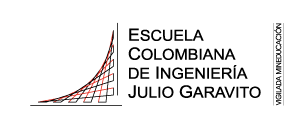
\includegraphics[scale=0.5]{Images/1110_logotipo_institucional_vm300px.png} \\
		    \Large{\textbf{Escuela Colombiana de Ingeniería Julio Garavito}\vspace{2cm}}\\
		    \textbf{Maestría en Gestión de Información}\vspace{1cm}\\
		    \textbf{Ley en Gestión de Información}\vspace{1cm}\\
			\textsc{Taller 1} \vspace{2cm}  \\   
			\emph{Autor:} \textit{Ing. Fabio Quintero}\vspace{5cm}\\
	     \textit{\today}\\

	   \end{center}
	   \vspace*{\stretch{2.0}}
	\end{titlepage}
	






\section{Derechos de Autor}

\subsection{Participación ciudadana}


\subsection{Participación como opción de grado}


\section{Protección de datos}
\subsection{Acceso a la información pública}
Acorde la ley de acceso de transferencia y del derecho a acceso a la información pública \footnote{Ley 1712 de 2014} las UGPP y la DIAN está obligados como se expresa en el Artiículo 5 literal a toda entidad pública a todos los niveles, siendo así se podría solicitar toda la información requerida sin perjucio y/o explicación alguna por parte del requieriente, pero teniendo en cuenta el caso planteado y como se explica en la subsiguiente sección ~\ref{subsec:semiprivados} los datos que la DIAN en calidad de Operador de la información \citep{Ley12662008}\footcite{Articulo 3\grad, Definiciones}, obtuvo esta información pro de cumplir su misión insitucional, es decir garantizar que todos los habitantes del territorio Colombiano cumplan con sus obligaciones tributarias, siendo así la información generada por la UGPP de un titular es de interés de la DIAN para el cumplimiento tributario del mismo a lo cual implica que esta información privada se convierte en semiprivada por definición.\citep{Ley12662008}\footcite{Artiículo 5, Definiciones - Dato Semiprivado}.
Por lo tanto si los datos en específico que se transfirieron entre estas 2 entidas son semiprovados, deberemos acudir LEY 1712 Artículo 6 literal \textit{c}, \textsc{Información pública clasificada}, donde se espcifica que esta información será pública clasificada por la naturaleza previamente descrita.
\\
Podemos concluir que cualquier ciudadano podrá solicitar la información que tenga a bien y que la DIAN y la UGPP con administradores deberán garantizar la privacidad de los titulares de la información y deberan entregar dicha información clasificada sin perjucio de la intimidad de los titulares.


\subsection{Datos semiprivados}
\label{subsec:semiprivados}
Teniendo en cuenta el Artículo 13 de la ley de protección de datos personales\footnote{Ley Estatutaria 1581 de 2012}, estas 2 entidades públicas están autorizadas a obtener y consultar la información de las personas que lo entiendan como necesario, por lo tanto no requieren hacer ninguna clase de solicitud, como pedir la autorización del titular de los datos.
\\
Si bien cualquier ciudadano tiene el derecho constitucional de que se garantice su intimidad ''Todas las personas tienen derecho a su intimidad personal y familiar y a su  buen nombre, y el Estado debe respetarlos y hacerlos respetar \dots''\footnote{Constitución Política de Colombia, Articulo 15}, la ley de hábeas data\footnote{Ley Estatutaria 1266 de 2008} es garante de regular la información crediticia, comercial y servicios entre otros, entonces el titular de la información acudirá a esta pensando que puede bloquear el intercambio de esta información entre la UGPP y la DIAN, es de aclarar que por normatividad la UGPP debe contar con la autorización del titular para el uso de datos privados, por lo tanto el titular podría pensar que esta autorización es solo para la UGPP y no la DIAN y que estas 2 entidades tiene misiones diferentes y no deberían poder usar los datos sin su autorización, pero la misionalidad de este intercambio de datos es garantizar que cualquier persona con las normas relacionadas al pago de impuestos y no los evada por lo tanto esta ley no impide que estos datos sean intercambiados.
\\
Se define un dato como semi privado ''Es semiprivado el dato que no tiene naturaleza íntima, reservada, ni pública y cuyo conocimiento o divulgación puede interesar no sólo a su titular sino a cierto sector o grupo de personas o a la sociedad en general, como el dato financiero y crediticio de actividad comercial o de servicios a que se refiere el Título IV de la presente ley''. Esta definición y lo anterior para hacer cumplir la función de la DIAN y que no exista alguien (incluyendo al titular) que evada impuestos los datos se convertirán en semiprivados.



%----------------------------------------------------------------------------------------
%	BIBLIOGRAPHY
%----------------------------------------------------------------------------------------

\printbibliography[heading=bibintoc]


\end{document}
